\documentclass{standalone}
\usepackage{tikz}
\usetikzlibrary{patterns, positioning}


\begin{document}
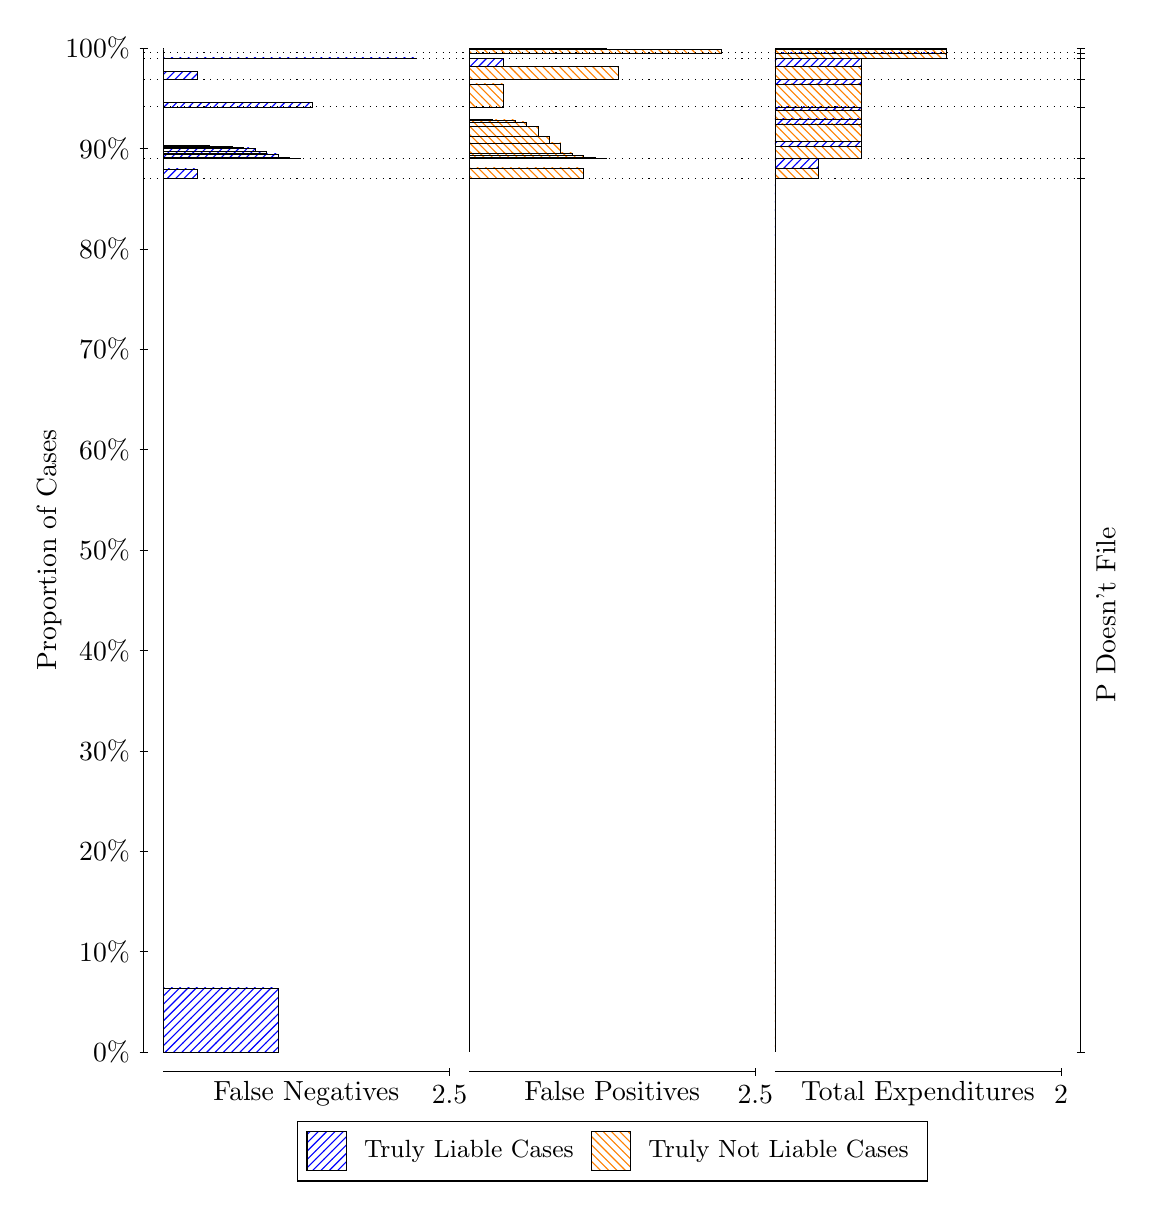
\begin{tikzpicture}
\draw[black, very thin] (1.5,1.75) -- (1.5,14.5);
\node[rotate=90, text=black, anchor=center] at (0.3, 8.125) {Proportion of Cases};
\draw[black, very thin] (1.45,1.75) -- (1.55,1.75);
\node[text=black, anchor=east] at (1.45, 1.75) {0\%};
\draw[black, very thin] (1.45,3.025) -- (1.55,3.025);
\node[text=black, anchor=east] at (1.45, 3.025) {10\%};
\draw[black, very thin] (1.45,4.3) -- (1.55,4.3);
\node[text=black, anchor=east] at (1.45, 4.3) {20\%};
\draw[black, very thin] (1.45,5.575) -- (1.55,5.575);
\node[text=black, anchor=east] at (1.45, 5.575) {30\%};
\draw[black, very thin] (1.45,6.85) -- (1.55,6.85);
\node[text=black, anchor=east] at (1.45, 6.85) {40\%};
\draw[black, very thin] (1.45,8.125) -- (1.55,8.125);
\node[text=black, anchor=east] at (1.45, 8.125) {50\%};
\draw[black, very thin] (1.45,9.4) -- (1.55,9.4);
\node[text=black, anchor=east] at (1.45, 9.4) {60\%};
\draw[black, very thin] (1.45,10.675) -- (1.55,10.675);
\node[text=black, anchor=east] at (1.45, 10.675) {70\%};
\draw[black, very thin] (1.45,11.95) -- (1.55,11.95);
\node[text=black, anchor=east] at (1.45, 11.95) {80\%};
\draw[black, very thin] (1.45,13.225) -- (1.55,13.225);
\node[text=black, anchor=east] at (1.45, 13.225) {90\%};
\draw[black, very thin] (1.45,14.5) -- (1.55,14.5);
\node[text=black, anchor=east] at (1.45, 14.5) {100\%};

\draw[black, very thin] (13.4,1.75) -- (13.4,14.5);
\draw[black, very thin] (13.35,1.75) -- (13.45,1.75);
\node[anchor=west] at (13.35, 1.75) {};
\draw[black, very thin] (13.35,12.848) -- (13.45,12.848);
\node[anchor=west] at (13.35, 12.848) {};
\draw[black, very thin] (13.35,13.094) -- (13.45,13.094);
\node[anchor=west] at (13.35, 13.094) {};
\draw[black, very thin] (13.35,13.753) -- (13.45,13.753);
\node[anchor=west] at (13.35, 13.753) {};
\draw[black, very thin] (13.35,14.1) -- (13.45,14.1);
\node[anchor=west] at (13.35, 14.1) {};
\draw[black, very thin] (13.35,14.37) -- (13.45,14.37);
\node[anchor=west] at (13.35, 14.37) {};
\draw[black, very thin] (13.35,14.439) -- (13.45,14.439);
\node[anchor=west] at (13.35, 14.439) {};
\draw[black, very thin] (13.35,14.5) -- (13.45,14.5);
\node[anchor=west] at (13.35, 14.5) {};

\draw[black, very thin, pattern color=blue, pattern=north east lines] (1.75,1.75) rectangle (3.2033,2.5637);
\draw[black, very thin, pattern color=orange, pattern=north west lines] (1.75,2.5637) rectangle (1.75,12.848);
\draw[black, very thin, pattern color=blue, pattern=north east lines] (1.75,12.848) rectangle (2.186,12.965);
\draw[black, very thin, pattern color=orange, pattern=north west lines] (1.75,12.965) rectangle (1.75,13.094);
\draw[black, very thin, pattern color=blue, pattern=north east lines] (1.75,13.094) rectangle (3.494,13.098);
\draw[black, very thin, pattern color=blue, pattern=north east lines] (1.75,13.098) rectangle (3.3487,13.114);
\draw[black, very thin, pattern color=blue, pattern=north east lines] (1.75,13.114) rectangle (3.2033,13.156);
\draw[black, very thin, pattern color=blue, pattern=north east lines] (1.75,13.156) rectangle (3.058,13.158);
\draw[black, very thin, pattern color=blue, pattern=north east lines] (1.75,13.158) rectangle (3.058,13.184);
\draw[black, very thin, pattern color=blue, pattern=north east lines] (1.75,13.184) rectangle (2.9127,13.232);
\draw[black, very thin, pattern color=blue, pattern=north east lines] (1.75,13.232) rectangle (2.7673,13.242);
\draw[black, very thin, pattern color=blue, pattern=north east lines] (1.75,13.242) rectangle (2.622,13.251);
\draw[black, very thin, pattern color=blue, pattern=north east lines] (1.75,13.251) rectangle (2.4767,13.254);
\draw[black, very thin, pattern color=blue, pattern=north east lines] (1.75,13.254) rectangle (2.3313,13.259);
\draw[black, very thin, pattern color=orange, pattern=north west lines] (1.75,13.259) rectangle (1.75,13.753);
\draw[black, very thin, pattern color=blue, pattern=north east lines] (1.75,13.753) rectangle (3.6393,13.809);
\draw[black, very thin, pattern color=orange, pattern=north west lines] (1.75,13.809) rectangle (1.75,14.1);
\draw[black, very thin, pattern color=blue, pattern=north east lines] (1.75,14.1) rectangle (2.186,14.2);
\draw[black, very thin, pattern color=orange, pattern=north west lines] (1.75,14.2) rectangle (1.75,14.37);
\draw[black, very thin, pattern color=blue, pattern=north east lines] (1.75,14.37) rectangle (4.9473,14.375);
\draw[black, very thin, pattern color=orange, pattern=north west lines] (1.75,14.375) rectangle (1.75,14.439);
\draw[black, very thin, pattern color=orange, pattern=north west lines] (1.75,14.439) rectangle (1.75,14.48);
\draw[black, very thin, pattern color=blue, pattern=north east lines] (1.75,14.48) rectangle (1.75,14.5);
\draw[black, very thin, pattern color=orange, pattern=north west lines] (5.6333,1.75) rectangle (5.6333,12.035);
\draw[black, very thin, pattern color=blue, pattern=north east lines] (5.6333,12.035) rectangle (5.6333,12.848);
\draw[black, very thin, pattern color=orange, pattern=north west lines] (5.6333,12.848) rectangle (7.0867,12.977);
\draw[black, very thin, pattern color=blue, pattern=north east lines] (5.6333,12.977) rectangle (5.6333,13.094);
\draw[black, very thin, pattern color=orange, pattern=north west lines] (5.6333,13.094) rectangle (7.3773,13.103);
\draw[black, very thin, pattern color=orange, pattern=north west lines] (5.6333,13.103) rectangle (7.232,13.111);
\draw[black, very thin, pattern color=orange, pattern=north west lines] (5.6333,13.111) rectangle (7.0867,13.137);
\draw[black, very thin, pattern color=orange, pattern=north west lines] (5.6333,13.137) rectangle (6.9413,13.168);
\draw[black, very thin, pattern color=orange, pattern=north west lines] (5.6333,13.168) rectangle (6.796,13.295);
\draw[black, very thin, pattern color=orange, pattern=north west lines] (5.6333,13.295) rectangle (6.6507,13.373);
\draw[black, very thin, pattern color=orange, pattern=north west lines] (5.6333,13.373) rectangle (6.5053,13.509);
\draw[black, very thin, pattern color=orange, pattern=north west lines] (5.6333,13.509) rectangle (6.36,13.561);
\draw[black, very thin, pattern color=orange, pattern=north west lines] (5.6333,13.561) rectangle (6.2147,13.588);
\draw[black, very thin, pattern color=blue, pattern=north east lines] (5.6333,13.588) rectangle (5.924,13.593);
\draw[black, very thin, pattern color=blue, pattern=north east lines] (5.6333,13.593) rectangle (5.7787,13.596);
\draw[black, very thin, pattern color=blue, pattern=north east lines] (5.6333,13.596) rectangle (5.6333,13.753);
\draw[black, very thin, pattern color=orange, pattern=north west lines] (5.6333,13.753) rectangle (6.0693,14.045);
\draw[black, very thin, pattern color=blue, pattern=north east lines] (5.6333,14.045) rectangle (5.6333,14.1);
\draw[black, very thin, pattern color=orange, pattern=north west lines] (5.6333,14.1) rectangle (7.5227,14.271);
\draw[black, very thin, pattern color=blue, pattern=north east lines] (5.6333,14.271) rectangle (6.0693,14.37);
\draw[black, very thin, pattern color=orange, pattern=north west lines] (5.6333,14.37) rectangle (5.6333,14.435);
\draw[black, very thin, pattern color=blue, pattern=north east lines] (5.6333,14.435) rectangle (5.6333,14.439);
\draw[black, very thin, pattern color=orange, pattern=north west lines] (5.6333,14.439) rectangle (8.8307,14.48);
\draw[black, very thin, pattern color=blue, pattern=north east lines] (5.6333,14.48) rectangle (7.3773,14.5);
\draw[black, very thin, pattern color=orange, pattern=north west lines] (9.5167,1.75) rectangle (9.5167,12.035);
\draw[black, very thin, pattern color=blue, pattern=north east lines] (9.5167,12.035) rectangle (9.5167,12.848);
\draw[black, very thin, pattern color=orange, pattern=north west lines] (9.5167,12.848) rectangle (10.062,12.977);
\draw[black, very thin, pattern color=blue, pattern=north east lines] (9.5167,12.977) rectangle (10.062,13.094);
\draw[black, very thin, pattern color=orange, pattern=north west lines] (9.5167,13.094) rectangle (10.607,13.255);
\draw[black, very thin, pattern color=blue, pattern=north east lines] (9.5167,13.255) rectangle (10.607,13.315);
\draw[black, very thin, pattern color=orange, pattern=north west lines] (9.5167,13.315) rectangle (10.607,13.536);
\draw[black, very thin, pattern color=blue, pattern=north east lines] (9.5167,13.536) rectangle (10.607,13.601);
\draw[black, very thin, pattern color=orange, pattern=north west lines] (9.5167,13.601) rectangle (10.607,13.713);
\draw[black, very thin, pattern color=blue, pattern=north east lines] (9.5167,13.713) rectangle (10.607,13.753);
\draw[black, very thin, pattern color=orange, pattern=north west lines] (9.5167,13.753) rectangle (10.607,14.045);
\draw[black, very thin, pattern color=blue, pattern=north east lines] (9.5167,14.045) rectangle (10.607,14.1);
\draw[black, very thin, pattern color=orange, pattern=north west lines] (9.5167,14.1) rectangle (10.607,14.271);
\draw[black, very thin, pattern color=blue, pattern=north east lines] (9.5167,14.271) rectangle (10.607,14.37);
\draw[black, very thin, pattern color=orange, pattern=north west lines] (9.5167,14.37) rectangle (11.697,14.435);
\draw[black, very thin, pattern color=blue, pattern=north east lines] (9.5167,14.435) rectangle (11.697,14.439);
\draw[black, very thin, pattern color=orange, pattern=north west lines] (9.5167,14.439) rectangle (11.697,14.48);
\draw[black, very thin, pattern color=blue, pattern=north east lines] (9.5167,14.48) rectangle (11.697,14.5);
\draw[black, dotted] (1.5,12.848) -- (13.4,12.848);
\draw[black, dotted] (1.5,13.094) -- (13.4,13.094);
\draw[black, dotted] (1.5,13.753) -- (13.4,13.753);
\draw[black, dotted] (1.5,14.1) -- (13.4,14.1);
\draw[black, dotted] (1.5,14.37) -- (13.4,14.37);
\draw[black, dotted] (1.5,14.439) -- (13.4,14.439);
\draw[black, very thin] (1.75,1.5) -- (5.3833,1.5);
\node[text=black, anchor=north] at (3.5667, 1.5) {False Negatives};
\draw[black, very thin] (5.3833,1.45) -- (5.3833,1.55);
\node[text=black, anchor=north] at (5.3833, 1.45) {2.5};

\draw[black, very thin] (5.6333,1.5) -- (9.2667,1.5);
\node[text=black, anchor=north] at (7.45, 1.5) {False Positives};
\draw[black, very thin] (9.2667,1.45) -- (9.2667,1.55);
\node[text=black, anchor=north] at (9.2667, 1.45) {2.5};

\draw[black, very thin] (9.5167,1.5) -- (13.15,1.5);
\node[text=black, anchor=north] at (11.333, 1.5) {Total Expenditures};
\draw[black, very thin] (13.15,1.45) -- (13.15,1.55);
\node[text=black, anchor=north] at (13.15, 1.45) {2};

\node[text=black, centered, rotate=90] at (13.72, 7.2991) {P Doesn't File};







\draw (7.449999999999999,1.5) node[draw=none] (baseCoordinate) {};
\begin{scope}[align=center]
        \matrix[scale=0.5, draw=black, below=0.5cm of baseCoordinate, nodes={draw}, column sep=0.1cm]{
            \node[rectangle, draw, minimum width=0.5cm, minimum height=0.5cm, pattern color=blue, pattern=north east lines] {}; &
            \node[draw=none, font=\small, text=black] (B) {Truly Liable Cases}; &
            \node[rectangle, draw, minimum width=0.5cm, minimum height=0.5cm, pattern color=orange, pattern=north west lines] {}; &
            \node[draw=none, font=\small, text=black] (B) {Truly Not Liable Cases}; \\
            };
\end{scope}

\end{tikzpicture}
\end{document}